\clearpage

\section {Neutrino oscillation fitting}
\label{sec:oscfit}

%--------------------------------------------------------------------------------------------------------------------
\subsection {Fitting methodology}
\label{sec:oscfit_method}

%....................................................................................................................
\subsubsection {Choice of 23-sector oscillation parameters}
\label{sec:oscfit_method_23param_choice}

Several choices exist for the 23-sector oscillation parameters that could be fitted, 
and they have been presented in the context of the VaLOR joint 3-flavour oscillation analysis \cite{Lorena}.
The mixing parameter typically fitted is $\sin^{2}2\theta_{23}$, 
but $\sin^{2}\theta_{23}$ is a more natural choice in the context of a 3-flavour analysis,
especially one with any sensitivity to resolve the octant degeneracy.
The mass-squared difference typically fitted is $|\Delta m^{2}_{32}|$; this is the largest squared-mass splitting for the inverted mass
hierarchy but the second largest for the normal mass hierarchy. 
It is therefore not correct to compare results obtained under the different mass hierarchy hypotheses.
Other choices include fitting for a mass-squared difference whose absolute value is the same for both mass hierarchies,
such as $\Delta m^{2} = \left(m_{3}^{2} - \frac {m_{1}^{2}+m_{2}^{2}} {2} \right)$ \cite{FogliLisi},
or fitting for $|\Delta m^{2}_{32}|$ for the inverted hierarchy and $|\Delta m^{2}_{31}|$ for the normal hierarchy \cite{GonzalezGarcia}.
All these choices are implemented in the VaLOR oscillation analysis framework, and our analysis can switch between them.

For the Run 1+2+3 datasets, it was agreed that all official T2K $\nu_{\mu}$-disappearance analyses will continue 
to fit the usual parameters $\sin^{2}2\theta_{23}$ and $|\Delta m^{2}_{32}|$.

The PRL referees requested that we present the result in terms of $\sin^2\theta_{23}$ and $|\Delta m^{2}_{32}|$,
so the result for this variable has been added to the note.
The fact that the the center of symmetry (point of maximal disappearance) is not at $\sin^2\theta_{23} = 0.5$ makes this a sensible choice.

%....................................................................................................................
\subsubsection {Treatment of non-23-sector oscillation parameters}
\label{sec:oscfit_method_non23params}

In a 3-flavour $\nu_{\mu}$-disappearance fit, it is also necessary to make a choice for the non-23 oscillation parameters. 
Possible options for these parameters include
\begin{enumerate}
\item All 6 parameters, i.e. $\sin^{2}(2 \theta_{12})$, $\sin^{2}(2 \theta_{13})$, $\sin^{2}(2 \theta_{23})$, $\Delta m_{21}^{2}$,
$|\Delta m_{32}^{2}|$ and $\delta_{CP}$ can float freely.
\item All 6 parameters can float freely, but deviations in values of $\sin^{2}(2 \theta_{12})$, $\sin^{2}(2 \theta_{13})$ and
$\Delta m_{21}^{2}$ from values measured by other experiments are penalised.
\item $\sin^{2}(2 \theta_{23})$ and $|\Delta m_{32}^{2}|$ can float freely, but $\sin^{2}(2 \theta_{12})$, $\sin^{2}(2 \theta_{13})$,
$\Delta m_{21}^{2}$ and $\delta_{CP}$ are fixed.
\end{enumerate}

In the present analysis, option 3 is used. 
When finding the best-fit values of $\sin^{2}(2 \theta_{23})$ and $|\Delta m_{32}^{2}|$,
the values of $\Delta m_{21}^{2}$, $\sin^{2}(2 \theta_{12})$ and $\sin^{2}(2 \theta_{13})$
are fixed to the 2012 PDG best-fit values \cite{PDG2012} shown in Tab.\ \ref{tab:pdg2012non23},
and $\delta_{CP}$ is fixed to 0.

\begin{table}
\centering
\begin{tabular}{| c | c | c | }
\hline
Parameter                  &  Best-fit                                    & 1$\sigma$ error  \\
\hline
$\Delta m_{21}^{2}$        &  7.5 $\times$ 10$^{-5}$ eV$^{2}$/c$^{4}$     & $\sim$3\% \\
$\sin^{2}(2 \theta_{12})$  &  0.857                                       & $\sim$3\% \\
$\sin^{2}(2 \theta_{13})$  &  0.098                                       & $\sim$13\% \\
\hline
\end{tabular}
\caption{
  2012 PDG best-fit values and 1$\sigma$ range for the measured non-23-sector oscillation parameters \cite{PDG2012}.
}
\label{tab:pdg2012non23}
\end{table}


%The uncertainties due to uncertain values of the non-23 oscillation parameters are incorporated into the confidence countours. This is done
%by randomly varying the non-23 parameters when creating the toy Monte Carlo datasets used to find the critical values of $\Delta \chi^{2}$ at
%each point in the oscillation parameter grid (see section \ref{sec:contour_construction_fc}).

%....................................................................................................................
\subsubsection {Treatment of systematic parameters}
\label{sec:oscfit_method_nuisance}

In this analysis, 48 nuisance (systematic) parameters are taken into account 
in the prediction of the single $\mu$-like ring event reconstructed energy spectrum (see Sec.\ \ref{sec:systematics}).
{\bf The VaLOR group produces oscillation results including all nuisance parameters in the fit}.

At the time of the muon-neutrino disappearance analysis of the Run1+2 dataset, 
the authors of this analysis (at that time referred to as the Rutherford/Oxford analysis \cite{OurRun12DisappAnalysis}) 
took the view that, due to low statistics, and in the interest of simplicity and robustness, 
fitting for all the numerous systematic parameters considered in the analysis was not warranted.
It was shown that fitting for no systematics obtained results which were very similar to the ones
obtained by fitting for all systematics.
It was argued that better services would be provided to the community by focussing our paper on the
power of the off-axis technique rather than on statistical gymnastics.
Most T2K collaborators shared this view, and the Rutherford/Oxford result was chosen as the
primary result shown in the first muon-neutrino disappearance paper \cite{T2KRun12Disapp}.
Similar views may be expressed in the context of the present analysis.
Due to a two-fold increase of the integrated exposure since the time of the Run1+2 analysis,
fitting some of the dominant systematic parameters is now justified.
However, again, we express concerns that fitting for all 48 systematic parameters 
considered in this analysis is not warranted,
especially in view of the small effect many of them have 
compared with the effect of some of the approximations made in this analysis.
We have therefore sought to reduce the dimensionsality of our fit
while accounting for the full systematic effects on our measurements of
$\sin^{2}{2\theta_{23}}$ and $|\Delta m^{2}_{32}|$. 
{\bf In addition to the result obtained by fitting all systematics, 
the VaLOR group produces {\em alternative} oscillation results by allowing only 
the most important systematics to float in the fit}.
A detailed study to select the systematic parameters to include in the 
fit for the alternative result is presented in Sec.\ \ref{sec:fit_syst_analysis}.
We give the VaLOR group viewpoint on which is the preferred result to show publicly
in Sec.\ \ref{sec:primary_result_selection}, after presenting all the results in detail.

%....................................................................................................................
\subsubsection {Allowed range of fit parameters}
\label{sec:oscfit_method_param_range}

The search for the minimum value of 
$-2 \, \textrm{ln} \lambda(\sin^{2}2\theta_{23},|\Delta m^ {2}_{32}|; {\bf a})$ (see Eq. \ref{eq:chisquare}) 
is performed in the range 
$0 \leq$ $\sin^{2}2\theta_{23}$ $\leq 1$ and
$1 \times 10^{-3} eV^{2}/c^{4} \leq$ $|\Delta m^{2}_{32}|$ $\leq 6 \times 10^{-3} eV^{2}/c^{4}$.
Values of $\sin^{2}2\theta_{23}$ $> 1$  are not permitted; although it is numerically allowed and,
occasionally, it yields better fits to data, it has no physical interpretation within the context
in which we attempt to interpret the data and causes p.d.f.s to have pathological behaviour.

Systematic parameters included in the oscillation fit are constrained in the range [-5$\sigma_{s}$, +5$\sigma_{s}$]
where $\sigma_{s}$ is the one standard deviation error assigned to each systematic parameter\footnote{
 Such an error is defined for all but one of the systematic parameters considered in this analysis. 
 The exception is the systematic parameter $f_{SF}$ which parameterizes the uncertainty on nuclear modelling, 
 switching between the Relativistic Fermi Gas (RFG) and Spectral Function (SF) models. The allowed range of the parameter $f_{SF}$ 
in the oscillation fit is [0,1].}.
Values of systematic parameters that give a negative predicted number of events in any reconstructed energy bin are not allowed. 
If this scenario arises, the number of events is changed to +1E-8 in that bin. This is done for the sum of all the interaction 
modes rather than for each mode separately.

%....................................................................................................................
\subsubsection {Minimization method}
\label{sec:oscfit_method_chisq}

The VaLOR disappearance analysis uses a binned likelihood-ratio method.
Measurements of the oscillation parameters $\sin^{2}2\theta_{23}$ and $|\Delta m^{2}_{32}|$
are obtained by comparing the observed and predicted SuperK reconstructed energy spectra
for 1-ring $\mu$-like events.
Let $N$ be the number of reconstructed energy bins and
${\bf a}$ be a $1 \times N_{s}$ - dimensional array of systematic (nuisance) 
parameters that affect the SuperK reconstructed energy spectrum prediction (e.g
parameters that control the beam, neutrino interaction simulations and 
the detector response).
Best-fit values are obtained by minimizing: 
\begin{equation}
\displaystyle
%\chi^{2} 
-2 \, \textrm{ln} \lambda (\sin^{2}2\theta_{23},|\Delta m^{2}_{32}|; {\bf a}) = 
  2 \cdot \sum_{i=0}^{N-1} 
   \Big( 
     n^{obs}_{i} \cdot ln(n^{obs}_{i}/n^{exp}_{i}) +
     (n^{exp}_{i}-n^{obs}_{i}) 
   \Big) +
   ({\bf a}-{\bf a_{0}})^{T} \cdot {\bf C}^{-1} \cdot ({\bf a}-{\bf a_{0}})
\label{eq:chisquare}
\end{equation}
where
${\bf a_{0}}$ is an $1 \times N_{s}$ - dimensional array with the default values of 
the systematics parameters, ${\bf a}^{T}$ is the transpose of ${\bf a}$,
${\bf C}$ is the systematic parameter covariance matrix of dimension $N_{s} \times N_{s}$,
$n^{obs}_{i}$ is the observed number of events in the $i^{th}$ bin, and
$n^{exp}_{i} = n^{exp}_{i}(\sin^{2}2\theta_{23},|\Delta m^{2}_{32}|; {\bf a})$ 
is the corresponding expected number of events.

The likelihood-ratio method used in this analysis, is equivalent to the extended maximum likelihood
method used in the alternative T2K oscillation analysis 
(see \cite{OurRun1DisappAnalysis,StatAnalysisCowan} for more details).
The advantage of the likelihood ratio method, compared with the extended maximum-likelihood method, is that
in the large-sample limit, the quantity $-2 \, \textrm{ln} \lambda (\sin^{2}2\theta_{23},|\Delta m^{2}_{32}|; {\bf a})$
in Eq.\ref{eq:chisquare} has a $\chi^{2}$ distribution and it can therefore be used as a goodness-of-fit test.
In this note
$-2 \, \textrm{ln} \lambda (\sin^{2}2\theta_{23},|\Delta m^{2}_{32}|; {\bf a})$ and
$\chi^{2}(\sin^{2}2\theta_{23},|\Delta m^{2}_{32}|; {\bf a})$ are used interchangeably.

The minimization is performed with Minuit \cite{Minuit}, using the Migrad method.
If Migrad does not converge, the starting values of the oscillation parameters are re-initialised:
the new initial values are randomly drawn from uniform distributions in the ranges 
0.80 $\leq$ sin$^{2}2\theta_{23}$ $\leq$ 0.98, 
$2 \cdot 10^{-3}$ $\leq$ $|\Delta m^{2}_{32}|$ $\leq$ $3 \cdot 10^{-3}$
and the fit is retried. This is repeated 10 times.
If the fits still fail to converge, the Simplex algorithm is used.
The Hesse algorithm is called after a successful fit to improve Minuit's estimates of the
errors on the fitted parameters.

%....................................................................................................................
\subsubsection {Brief note on out fit labeling scheme}
\label{sec:oscfit_method_label}

In the following sections, the different fits are labeled as `$I_{osc}$+$I_{syst}$', 
where $I_{osc}$ and $I_{syst}$ represent, respectively, the number of oscillation and systematic
parameters which are allowed to float in the fit.
If the symbol N is shown in place of $I_{syst}$, all of the systematic parameters are allowed to float.
If an actual number is shown in place of $I_{syst}$, this is the number of systematics that is allowed to float.

Accoring to the above scheme, 
`2+N' denotes a fit of $\sin^{2}2\theta_{23}$, $|\Delta m^{2}_{32}|$ and all nuisance parameters, 
`2+8' denotes a fit of $\sin^{2}2\theta_{23}$, $|\Delta m^{2}_{32}|$ and the 8 most important systematic parameters,
`0+N' denotes a fit of all nuisance parameters with all oscillation parameters fixed, etc.

%....................................................................................................................
\subsection {Goodness-of-fit tests}
\label{sec:gof_test}

In our $\nu_{\mu}$-disappearance analysis of the Run1+2 datasets, p-values were computed using both 
a) the rate of single $\mu$-like ring events and 
b) the rate and reconstructed energy distribution of single $\mu$-like ring events using the likelihood-ratio method \cite{NickPvalue}.
The choice is not unique.

D. Karlen has pointed out that, if the statistics are low, "the use of the
distribution is not helpful in forming the p-value. 
This is directly related to the well known problem that is difficult to define
a general goodness-of-fit for sparsely populated distributions.
Large bins (or in the extreme a single bin = rate-only)
are necessary for small statistics samples" \cite{KarlenPvalue}.

It was decided by the oscillation analysis group that, for all $\nu_{\mu}$-disappearance analyses, 
p-values will be calculated using the rate and the reconstructed energy distribution,
and that the distribution will use a very coarse binning
scheme to ensure that there are sufficient numbers of events in each bin: 
this scheme has 5 bins from 0-0.4, 0.4-0.7, 0.7-1.0, 1.0-2.0 and 2.0-30.0 GeV.

%....................................................................................................................
\subsection {Toy Monte Carlo study of fitter performance}
\label{sec:toy_mc_fitter_performance}

The performance of the fitter was evaluated using an ensemble of 10k toy MC experiments, 
generated with input oscillation parameters $\sin^{2}2\theta_{23}$ = 0.9 and 
$|\Delta m^{2}_{32}|$ = 2.4$\times$10$^{-3}$ eV$^{2}$/c$^{4}$ and an exposure of 3.010$\times$10$^{20}$ POT.  
A further 10k toy MC experiments with the same input oscillation parameters and an exposure of
3.010$\times$10$^{22}$ POT (100 $\times$ Run1+2+3 exposure) were also used.
These simulated experiments included statistical fluctuations and fluctuations of the 8 dominant systematic 
parameters only (see Sec.\ \ref{sec:fit_syst_analysis}). 
The toy MC experiments were fitted using MINUIT and HESSE errors, with a `2+8' fit being used. 
Residual and pull distributions were studied for oscillation and systematic paraneters.
%After fitting, pulls were calculated for the oscillation parameters as follows:
%\begin{equation}
%\textrm{Pull}_{\textrm{\footnotesize{osc}}} = \frac{\textrm{Best fit parameter - input parameter}}{\sigma_{\textrm{\small{fit}}}}
%\end{equation}
%Pulls were also calculated for the 8 fitted systematic parameters:
%\begin{equation}
%\textrm{Pull}_{\textrm{\footnotesize{syst}}} = \frac{\textrm{Best fit parameter - input parameter}}
%{\sqrt{\sigma_{\textrm{\small{prior}}}^{2} - \sigma_{\textrm{\small{fit}}}^{2}}}
%\end{equation}
No issue was identified regarding the fitter performance, which was as expected
The results are presented in Appendix \ref{sec:appendix:fitter_performance}\footnote{
  Fitter performance tests have not been repeated for the fit in terms of $\sin^2\theta_{23}$,
  however they are available for similar analyses using the same code,
  in reference \cite{OurRun123JointOscillationAnalysis} for the joint oscillation analysis,
  fitting for $\sin^2\theta_{23}$ to Run 1-3 POT,
  and in reference \cite{OurRun1234aDisappAnalysis3Flavour} for the
  disappearance-only analysis, fitting for $\sin^2\theta_{23}$ to Run 1-4a POT.
  Both of these analyses use a (slightly) different systematic parameter representation,
  and also fit for some non-23-sector oscillation parameters.
  No problems have been found with the fitter performance in these cases.
}.

%....................................................................................................................
\subsection {Systematic analysis}
\label{sec:fit_syst_analysis}

This section describes a study into the effect of systematic uncertainties in the joint estimation of the
$\sin^{2}2\theta_{23}$ and $|\Delta m^{2}_{32}|$ using the fitting procedure described in Sec.\ \ref{sec:oscfit_method_chisq}. 
Only a summary is given here, and the full study is shown in Appendix \ref{appendix:systematics_bestfit_oscillations}.

To quantify the effect of each systematic, toy MC datasets are generated with no statistical fluctuations
and with the systematic parameter in question varied by $\pm$1$\sigma$. A `2+0' fit is performed on each dataset.
For correlated systematic parameters, $\sigma$ is defined as the square root of the 
corresponding covariance matrix diagonal element.
The effect of the systematic parameter on the oscillation parameters, for the given systematic parameter variation
and the input true oscillation point, is taken to be the difference between the best-fit and true oscillation points.

Figs.\ \ref{fig:star_important_0.80_0.0024}-\ref{fig:star_important_1.00_0.0030} 
show the so-called ``star plots'', 
which have arrows plotted for each systematic parameter from the true input point to the best-fit points for both the +1$\sigma$ 
and the -1$\sigma$ fits.
These figures show only the ``dominant'' systematic parameters,
which are defined as those having an effect on
$\sin^{2}2\theta_{23}$ and $|\Delta m^{2}_{32}|$ greater than 25\% of the expected statistical error 
at one or more true oscillation points in the area of interest in the parameter space.
The statistical error was evaluated using 10k toy MC datasets with no systematic fluctuations at each input point, 
with each dataset being fitted with the `2+0' method.
The maximum deviation found between the true input and best-fit oscillation parameters for all true oscillation points tested
is summarised in Tab.\ \ref{tab:star_summary}. 
The dominant systematic parameters are highlighted in red in that table.

The purpose of this study was to identify the dominant systematics in order to reduce
the dimensionality of the fit. As shown in Tab.\ \ref{tab:star_summary}, 
only 8 (out of a total of 48) systematic parameters have an effect which is larger than
25\% of the expected statistical error anywhere in the oscillation parameter space of interest.
These systematic parameters are:
\begin{itemize}
\item
$f_{E; r}^{SK}$: 
SuperK reconstructed energy scale systematic.
\item
$f_{CCnonQE; r}^{SK}$: 
$\nu_\mu$, $\bar{\nu}_{\mu}$ SuperK CCnonQE efficiency systematic.
This is a combined systematic parameter which includes the uncertainty on all 
fiducial volume, ring-counting, reduction chain, OD cut, PID cut, momentum cut and decay electron cut efficiencies.
\item
$f_{NC; r}^{SK}$:
SuperK NC efficiency systematic.
This is a combined systematic parameter which includes all sources of uncertainty listed above for $f_{CCnonQE; r}^{SK}$.
\item
$f_{16; t, r}^{banff}$:
CCQE axial mass systematic.
\item
$f_{18; t, r}^{banff}$:
CCQE normalisation systematic in the true energy range 0 - 1.5 GeV.
\item
$f_{bindE; t, r}$:
$^{16}O$ binding energy systematic.
\item
$f_{SF; t, r}$:
$^{16}O$ nuclear environment modeling systematic. Switches from Fermi Gas (RFG) to Spectral Function (SF) model.
\item
$f_{\pi-less\Delta; t, r}$:
Systematic parameter taking into account the uncertainty in the fraction 
of $\pi$-less $\Delta$ decays is resonance neutrino-production events.
\end{itemize}

When performing a '2+8' fit, it should be noted that correlations are
respected; the 21 BANFF parameters which are not fitted move as a result
of changing the 2 BANFF parameters which are fitted,
and all BANFF parameters contribute to the fit penalty term.
Also, it should be noted that all parameter correlations are taken
into account when the toy MC experiments are generated, and this is
true for all fit methods.

It was decided to perform a `2+8' oscillation fit in addition to the `2+N' fit, 
This was done with the underlying assumption that, if the results of the two fits were identical, 
the `2+8' fit would be the preferred one to present outside T2K due
to its simpicity, robustness, economy of assumptions and ease of explanation.
It is physically correct and accounts for the full
systematic error on our measurements. 


\begin{figure*}[htb]
\begin{minipage}[t]{0.48\linewidth}
\center
\includegraphics[width=18pc]{{./images/star_plot/important-0.800000-0.002400_testbig}.eps}
\caption {Effects of variation by $\pm1\sigma$ of the 8 dominant systematic parameters
  on the oscillation parameters $\sin^{2}2\theta_{23}$ and $|\Delta m^{2}_{32}|$.
  The method used for estimating the systematic shift is described in Sec.\ \ref{sec:fit_syst_analysis}.
  The ellipse shown is one quarter the size of the statistical error. 
  The true 23-sector oscillation parameters used are 
  $\sin^{2}2\theta_{23}$ = 0.80 and $|\Delta m^{2}_{32}|$ = 2.4$\times10^{-3} eV^{2}/c^{4}$.
  The 2012 PDG values are used for $\sin^{2}2\theta_{13}$, $\sin^{2}2\theta_{12}$ and $\Delta m^{2}_{21}$,
  and $\delta_{CP}$=0. The normal mass hierarchy is assumed.
}
\label{fig:star_important_0.80_0.0024}
\end{minipage}
\hspace{0.06\linewidth}
\begin{minipage}[t]{0.48\linewidth}
\center
\includegraphics[width=18pc]{{./images/star_plot/important-0.950000-0.002400_testbig}.eps}
\caption { 
  As in Fig.\ \ref{fig:star_important_0.80_0.0024},
  but for true 23-sector oscillation parameters 
  $\sin^{2}2\theta_{23}$ = 0.95 and $|\Delta m^{2}_{32}|$ = 2.4$\times10^{-3} eV^{2}/c^{4}$.
}
\label{fig:star_important_0.95_0.0024}
\end{minipage}
\vfill
\begin{minipage}[t]{0.48\linewidth}
\center
\includegraphics[width=18pc]{{./images/star_plot/important-1.000000-0.002400_testbig}.eps}
\caption { 
  As in Fig.\ \ref{fig:star_important_0.80_0.0024},
  but for true 23-sector oscillation parameters 
  $\sin^{2}2\theta_{23}$ = 1.00 and $|\Delta m^{2}_{32}|$ = 2.4$\times10^{-3} eV^{2}/c^{4}$.
}
\label{fig:star_important_1.00_0.0024}
\end{minipage}
\hspace{0.06\linewidth}
\begin{minipage}[t]{0.48\linewidth}
\center
\includegraphics[width=18pc]{{./images/star_plot/important-1.000000-0.003000_testbig}.eps}
\caption { 
  As in Fig.\ \ref{fig:star_important_0.80_0.0024},
  but for true 23-sector oscillation parameters 
  $\sin^{2}2\theta_{23}$ = 1.00 and $|\Delta m^{2}_{32}|$ = 3.0$\times10^{-3} eV^{2}/c^{4}$.
}
\label{fig:star_important_1.00_0.0030}
\end{minipage}
\end{figure*}

\clearpage

\begin{table}
\centering
\begin{tabular}{| c | c | c |}
\hline
 Parameter               &  $\frac{\delta_{syst} sin^22\theta_{23}}{\delta_{stat} sin^22\theta_{23}}$   &  $\frac{\delta_{syst}|\Delta m^2_{32}| (eV^{2}/c^{4})}{\delta_{stat} |\Delta m^2_{32}| (eV^{2}/c^{4})}$ \\
\hline

{\color{red}$f_{E; r}^{SK}$  }	 & 0.3486	 & 0.3058 \\
$f_{CCQEoth; r}^{SK}$	 & 0.0872	 & 0.0544 \\
$f_{CCQERC0; r}^{SK}$	 & 0.0106	 & 0.0099 \\
$f_{CCQERC1; r}^{SK}$	 & 0.1398	 & 0.1109 \\
$f_{CCQERC2; r}^{SK}$	 & 0.0686	 & 0.0741 \\
{\color{red}$f_{CCnQE; r}^{SK}$}	 & 0.3107	 & 0.2134 \\
{\color{red}$f_{NC; r}^{SK}$}	 & 1.1500	 & 0.6091 \\
$f_{\nu_e; r}^{SK}$	 & 0.0130	 & 0.0167 \\
$f_{0; t, r}^{banff}$	 & 0.0756	 & 0.0682 \\
$f_{1; t, r}^{banff}$	 & 0.0883	 & 0.1495 \\
$f_{2; t, r}^{banff}$	 & 0.0949	 & 0.1248 \\
$f_{3; t, r}^{banff}$	 & 0.0946	 & 0.0693 \\
$f_{4; t, r}^{banff}$	 & 0.2048	 & 0.1899 \\
$f_{5; t, r}^{banff}$	 & 0.1053	 & 0.0881 \\
$f_{6; t, r}^{banff}$	 & 0.0538	 & 0.0452 \\
$f_{7; t, r}^{banff}$	 & 0.0130	 & 0.0114 \\
$f_{8; t, r}^{banff}$	 & 0.0100	 & 0.0077 \\
$f_{9; t, r}^{banff}$	 & 0.0051	 & 0.0031 \\
$f_{10; t, r}^{banff}$	 & 0.0042	 & 0.0029 \\
$f_{11; t, r}^{banff}$	 & 0.0043	 & 0.0045 \\
$f_{12; t, r}^{banff}$	 & 0.0051	 & 0.0061 \\
$f_{13; t, r}^{banff}$	 & 0.0103	 & 0.0094 \\
$f_{14; t, r}^{banff}$	 & 0.0083	 & 0.0079 \\
$f_{15; t, r}^{banff}$	 & 0.0034	 & 0.0022 \\
{\color{red}$f_{16; t, r}^{banff}$}	 & 0.5979	 & 0.4068 \\
$f_{17; t, r}^{banff}$	 & 0.1557	 & 0.1067 \\
{\color{red}$f_{18; t, r}^{banff}$}	 & 0.4188	 & 0.2891 \\
$f_{19; t, r}^{banff}$	 & 0.0610	 & 0.0707 \\
$f_{20; t, r}^{banff}$	 & 0.0048	 & 0.0059 \\
$f_{21; t, r}^{banff}$	 & 0.2142	 & 0.1333 \\
$f_{22; t, r}^{banff}$	 & 0.0422	 & 0.0462 \\
$f_{pF; t, r}$	 & 0.0526	 & 0.0592 \\
{\color{red}$f_{bindE; t, r}$}	 & 0.3108	 & 0.3597 \\
{\color{red}$f_{SF; t, r}$}	 & 0.4914	 & 0.4249 \\
{\color{red}$f_{\pi-less\Delta; t, r}$}	 & 0.3358	 & 0.2342 \\
$f_{CCothShape; t, r}$	 & 0.0249	 & 0.0181 \\
$f_{Wshape; t, r}$	 & 0.0653	 & 0.0414 \\
$f_{CCcoh; t}$	 & 0.0348	 & 0.0301 \\
$f_{NC1\pi^\pm; t}$	 & 0.1282	 & 0.0941 \\
$f_{NCoth; t}$	 & 0.1083	 & 0.0858 \\
$f_{CC\nu_e; t}$	 & 0.0052	 & 0.0022 \\
$f_{CC\bar{\nu}; t}$	 & 0.1032	 & 0.0750 \\
$f_{0; t, r}^{FSI}$	 & 0.0056	 & 0.0020 \\
$f_{1; t, r}^{FSI}$	 & 0.0049	 & 0.0024 \\
$f_{2; t, r}^{FSI}$	 & 0.0054	 & 0.0022 \\
$f_{3; t, r}^{FSI}$	 & 0.1223	 & 0.0944 \\
$f_{4; t, r}^{FSI}$	 & 0.0059	 & 0.0100 \\
$f_{5; t, r}^{FSI}$	 & 0.0550	 & 0.0473 \\

\hline
\end{tabular}
\caption{
  Maximum deviations, as a fraction of statistical error at the oscillation parameter grid point, from the input values of 2+0 fits to datasets 
  with $\pm$1 sigma individual systematic variations at a 
  range of oscillation points. The 8 most important systematics are highlighted in red.
}
\label{tab:star_summary}
\end{table}

%--------------------------------------------------------------------------------------------------------------------
\subsection {Construction of confidence regions}
\label{sec:contour_construction}

In this analysis, we present confidence regions for all variations of the oscillation fit (`2+N' and `2+8').
Confidence regions are shown with both 
the constant $\Delta\chi^{2}$ (see Sec.\ \ref{sec:contour_construction_constdchi})
and the Feldman and Cousins (see Sec.\ \ref{sec:contour_construction_fc}) methods.
A definite recommendation on the preferred methodology for constructing confidence regions was provided by
the T2K $\nu_{\mu}$ contour committee \cite{T2KNuMuContourCom} and it will be reiterated in Sec.\ \ref{sec:primary_result_selection}.

The two methods have been described in detail in past T2K technical notes and presentations.
For completeness, we summarise both of these methods here
and provide definite statements on the exact methodology used for incorporating systematic errors.

The methods differ in the calculation of the critical values of $\Delta{\chi^{2}}$, which are used to identify the areas 
of the parameter space to be included in the allowed region for a given confidence level. This allowed region is
\begin{equation}
\displaystyle
\chi^{2}(\sin^{2}2\theta_{23},|\Delta m^{2}_{32}|; {\bf a}) < \chi_{min}^{2} + \Delta{\chi^{2}}_{critical}
\label{eq:chiconfregion}
\end{equation}

However, the procedure followed for constructing the $\chi^{2}$ surface itself,
as a function of $\sin^{2}2\theta_{23}$ and $|\Delta m^{2}_{32}|$, is common to both methods.
Assuming that N systematic parameters are allowed to float in the oscillation fit,
the values of $\chi^{2}(\sin^{2}2\theta_{23},|\Delta m^{2}_{32}|; {\bf a})$ 
are calculated via a `0+N' fit at {\em each} point of the (sin$^{2}$2$\theta_{23}$, $|\Delta$m$^{2}_{32}|$) 
2-dimensional grid, i.e.\ by fixing the oscillation parameters to the true values for the given grid point 
and minimising $\chi^{2}$ with respect to the N systematic parameters.

The following grid spacing is used in all confidence region construction methods:
$\delta{\sin^{2}2\theta_{23}}=5\times10^{-3}$ and
$\delta{|\Delta{m^{2}_{32}}|}=1\times10^{-4} eV^{2}/c^{4}$.
The $|\Delta{m^{2}_{32}}|$ binning is the same as that used in our Run 1+2 analysis,
while the $\sin^{2}2\theta_{23}$ bin size is reduced by 50\% since sensitivity studies showed
that the contour was expected to shrink in $\sin^{2}2\theta_{23}$ by a similar factor.

%....................................................................................................................
\subsubsection {Constant $\Delta\chi^{2}$ method}
\label{sec:contour_construction_constdchi}

The constant $\Delta\chi^{2}$ method for quoting uncertainties on parameters measured jointly
($\sin^{2}2\theta_{23}$, $|\Delta m^{2}_{32}|$ in our analysis) is described in \cite{PDG2012} (pp. 390-401).
It is a fully frequentist treatment using the Gaussian approximation.
One finds the best-fit point and calculates the confidence contours as lines of {\em constant} $\Delta{\chi^{2}}$
from this point\footnote{
For 1 fit parameter, the critical values of $\Delta{\chi^{2}}$ used are 
1.00 (68\% CL), 2.71 (90\% CL), 3.84 (95\% CL), 6.63 (99\% CL).
For 2 parameters fitted simultaneously, the critical values of $\Delta{\chi^{2}}$ used are 
2.30 (68\% CL), 4.61 (90\% CL), 5.99 (95\% CL), 9.21 (99\% CL).
}.

%....................................................................................................................
\subsubsection {Feldman and Cousins method}
\label{sec:contour_construction_fc}

The work of Feldman and Cousins \cite{FeldmanCousins} 
uses the freedom which is inherent in the Neyman construction of confidence regions
to address cases 
(in particular, cases with
Poisson processes with background and Gaussian errors near a physical boundary)
where classical construction of confidence regions produces overcoverage, undercoverage, or
in extreme cases, an empty region.

Using the Feldman and Cousins method, construction of the confidence region proceeds as follows: a number of toy MC experiment 
fits is performed for each point of the (sin$^{2}$2$\theta_{23}$, $|\Delta$m$^{2}_{32}|$) 2-dimensional grid.
For each grid point, the critical value of $\Delta\chi^{2}$ ($\Delta\chi^{2}_{critical}$)
is found such that $\alpha$ of the toy MC experiments have $\Delta\chi^{2}_{MC}$ $<$ $\Delta\chi^{2}_{critical}$,
where $\alpha$ is the desired confidence level.
The value of $\Delta\chi^{2}_{MC}$ for each toy MC experiment is calculated as
\begin{equation}
\displaystyle
\Delta \chi^{2}_{MC} = \chi^{2} \textrm{(true)} - \chi^{2} \textrm{(MC, best fit)}
\label{eq:deltachi2}
\end{equation}
where
``true'' means that the $\chi^{2}$ was computed using the true values of the oscillation parameters at that grid point, and
``best-fit'' means that the $\chi^{2}$ was computed using the actual best-fit values for that MC experiment.
The $\chi^{2}$ values are calculated using Eq. \ref{eq:chisquare}.

The Feldman and Cousins confidence regions for a fit to an actual dataset are drawn such that grid points 
with $\Delta\chi^{2}_{data}$ $<$ $\Delta\chi^{2}_{critical}$ are included within the contour, 
where $\Delta\chi^{2}_{data}$ is given by
\begin{equation}
\displaystyle
\Delta \chi^{2}_{data} = \chi^{2} \textrm{(true)} - \chi^{2} \textrm{(data, best fit)}
\label{qe:fccontour}
\end{equation} 

The principal difference between the Feldman and Cousins and the constant $\Delta\chi^{2}$ methods is that the former determines 
the value of $\Delta\chi^{2}_{critical}$ individually for each grid point, whereas the latter uses the same value 
for all grid points.

The Feldman and Cousins method does not  specify how systematics are to be included 
in the confidence region construction and different choices exist. 
To construct a 2-dimensional (sin$^{2}$2$\theta_{23}$, $|\Delta$m$^{2}_{32}|$) confidence region, 
where all N systematic parameters are included in the p.d.f. and all N systematics are allowed to float in the fit,
this analysis uses the following methodology: 
the value of $\Delta\chi^{2}_{critical}$ at each true (sin$^{2}$2$\theta_{23}$, $|\Delta$m$^{2}_{32}|$) grid point 
is calculated from an ensemble of toy MC experiments,
each one of which is generated with the true oscillation parameters of that point and with all N systematics randomised.
For each toy MC experiment,
a `2+N' fit is performed to obtain the value of $\chi^{2} \textrm{(MC, best fit)}$ used in Eq. \ref{eq:deltachi2}.
A separate `0+N' fit, with the oscillation parameters fixed to the true values, is performed to obtain the value of 
$\chi^{2} \textrm{(true)}$, i.e.\ $\chi^{2}$ is {\em independently} minimimised, for {\em each} toy MC experiment, with 
respect to the systematic parameters.
If only a subset M (M $<$ N) of the N systematics is allowed to float in the fit, all N systematics are again randomized 
in the generation of the datasets, and `2+M' and `0+M' fits are
performed to obtain $\chi^{2} \textrm{(MC, best fit)}$ and $\chi^{2} \textrm{(true)}$ respectively

In Fig.\ \ref{fig:fc_dchisqcrit_2d}, we show a Monte Carlo estimation using the Feldman-Cousins method
of the $\Delta\chi^{2}_{critical}$ values
used for calculation of the 68\% and 90\% CL confidence regions
for the $3.010 \times 10^{20}$-POT 3-flavour $\nu_{\mu}$-disappearance analysis
for both the `2+8' and `2+N' fit variants.
The surfaces were generated using an ensemble of toy MC experiments which included both
randomized systematic variations and statistical fluctuations.
Slices of the 2-dimensional distributions shown in Fig.\ \ref{fig:fc_dchisqcrit_2d},
are shown in Figs.\ \ref{fig:fc_dchisqcrit_slice_mixing} and \ref{fig:fc_dchisqcrit_slice_dmsq}.
From these $\Delta\chi^{2}_{critical}$ distributions, we anticipate that the confidence regions produced 
using the Feldman-Cousins method will be narrower along $|\Delta{m^{2}_{32}}|$ at maximal mixing than 
those made with the $\Delta\chi^{2}_{critical}$ method. The Feldman-Cousins contours will also be wider 
along $sin^{2}{2\theta_{23}}$ for values of $|\Delta{m^{2}_{32}}|$ near the best fit.

\begin{figure*}[htb]
\center
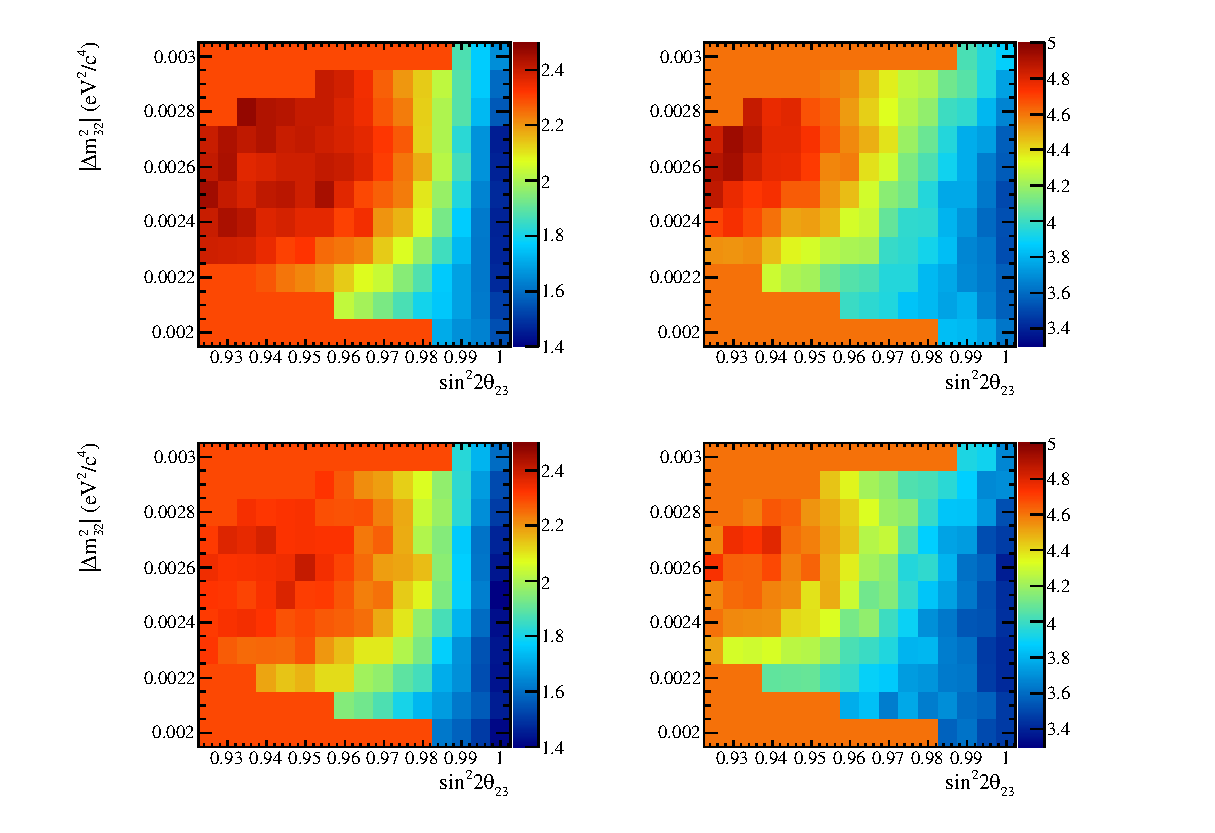
\includegraphics[width=42pc]{./images/feldman_cousins/FC_surfaces_28_2N.eps}
\caption {
  Monte Carlo estimation,
  according to the method of Feldman and Cousins,
  of $\Delta\chi^{2}_{critical}$ values $\Delta\chi^{2}_{68}$ (left) and $\Delta\chi^{2}_{90}$ (right)
  as functions of $\sin^{2}{2\theta_{23}}$ and $|\Delta{m^{2}_{32}}|$,
  for calculation of the 68\% and 90\% CL confidence regions
  for the 3.010 $\times$10$^{20}$-POT 3-flavour $\nu_{\mu}$-disappearance analysis.
  The top row shows $\Delta\chi^{2}_{critical}$ surfaces calculated using the `2+8' fit,
  whereas the bottom row shows surfaces calculated using the `2+N' fit.
  The surfaces were generated from an ensemble of toy-MC experiments including both
  randomized systematic variations and statistical fluctuations.
  As expected from \cite{FeldmanCousins}, the values of $\Delta\chi^{2}_{critical}$ 
  decrease as the physical boundary at $\sin^{2}{2\theta_{23}}$ = 1 is approached. 
}
\label{fig:fc_dchisqcrit_2d}
\end{figure*}

%.......

\begin{figure*}[htb]
\center
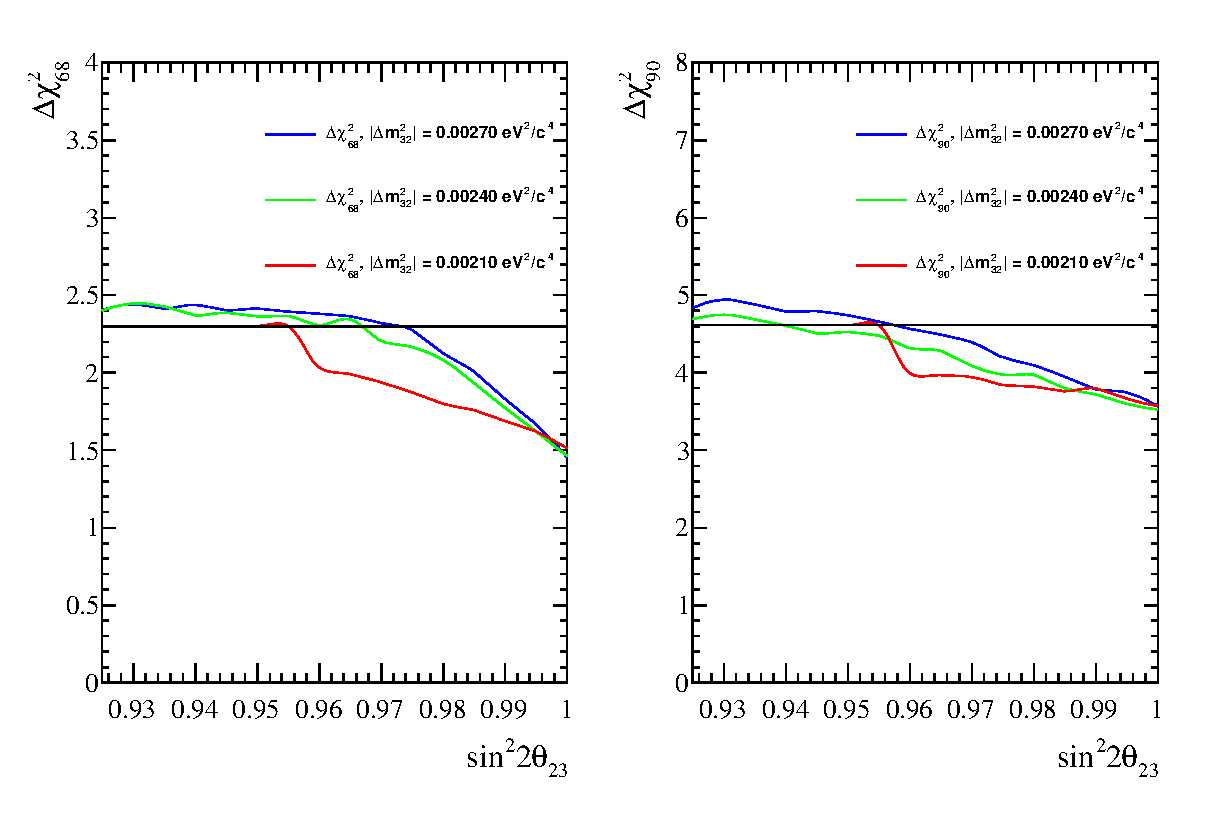
\includegraphics[width=30pc]{./images/feldman_cousins/FC_slice_mixing_28.eps}
\caption {
  Monte Carlo estimation,
  according to the method of Feldman and Cousins,
  of $\Delta\chi^{2}_{critical}$ values $\Delta\chi^{2}_{68}$ (left) and $\Delta\chi^{2}_{90}$ (right),
  as functions of $\sin^{2}{2\theta_{23}}$ for 3 different values of $|\Delta{m^{2}_{32}}|$
  (2.1$\times$10$^{-3}$ eV$^{2}/c^{4}$,
   2.4$\times$10$^{-3}$ eV$^{2}/c^{4}$ and
   2.7$\times$10$^{-3}$ eV$^{2}/c^{4}$).
  The $\Delta\chi^{2}_{critical}$ values were calculated
  from an ensemble of toy-MC experiments, for an exposure of 3.010$\times$10$^{20}$ POT, 
  including both randomized systematic variations and statistical fluctuations.
  The `2+8' fit was used.
  For comparison, the canonical value used in the constant $\Delta\chi^{2}_{critical}$
  method is also shown as a horizontal line.
}
\label{fig:fc_dchisqcrit_slice_mixing}
\end{figure*}

%.......

\begin{figure*}[htb]
\center
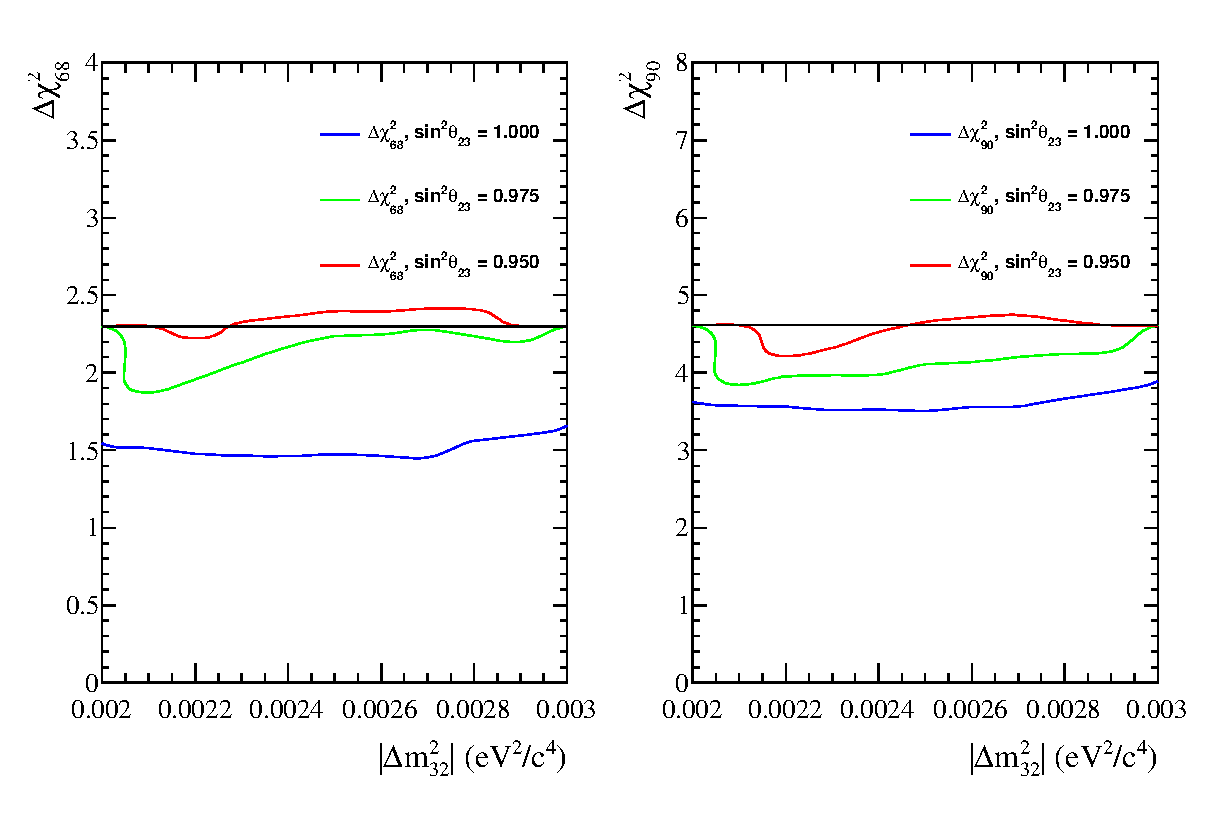
\includegraphics[width=30pc]{./images/feldman_cousins/FC_slice_dmsq_28.eps}
\caption {
  Monte Carlo estimation,
  according to the method of Feldman and Cousins,
  of $\Delta\chi^{2}_{critical}$ values $\Delta\chi^{2}_{68}$ (left) and $\Delta\chi^{2}_{90}$ (right),
  as functions of $|\Delta{m^{2}_{32}}|$ for 3 different values of $\sin^{2}{2\theta_{23}}$
  (0.950, 0.975 and 1.000).
  The $\Delta\chi^{2}_{critical}$ values were calculated
  from an ensemble of toy MC experiments, for an exposure of 3.010$\times$10$^{20}$ POT,
  including both randomized systematic variations and statistical fluctuations.
  The `2+8' fit was used.
  For comparison, the canonical value used in the constant $\Delta\chi^{2}_{critical}$
  method is also shown as a horizontal line.
}
\label{fig:fc_dchisqcrit_slice_dmsq}
\end{figure*}



